\documentclass[a4paper]{article}

\usepackage[T1]{fontenc}                % För svenska bokstäver
\usepackage[swedish]{babel}             % För svensk avstavning och svenska
                                        % rubriker (t ex "innehållsförteckning)
\usepackage[utf8]{inputenc}
\usepackage{ae}
\usepackage{graphicx}
\usepackage{url}

\usepackage{fancyvrb}
\fvset{tabsize=4}
\fvset{fontsize=\small}

\title{Projektplan}
%\author{Grupp 11}
\date{\today}

\begin{document}

\maketitle

\begin{center}

\large{Version 1.0}   			% Fyll i version!
\ \\[1cm]
\hrule
\ \\[1cm]
\begin{minipage}{0.5\textwidth}
	\begin{flushleft} \large
		\textbf{Gruppmedlemmar:} \\
		Reshad Ahmadi \\
		Maryam Bayat \\		
	\end{flushleft}
\end{minipage}

\begin{minipage}{0.4\textwidth}
	\begin{flushright} \large
		\textbf{Handledare:} \\
		Kenneth Nilsson \\
		\ \\				
		\textbf{Examinator:} \\
		Björn Åstrand
	\end{flushright}
\end{minipage}

\end{center}

\clearpage

\tableofcontents
\newpage

\section{Introduktion}
Detta projekt ämnat till att utveckla en Raviolimaskin. Ravioli är en traditionell italiensk maträtt bestående av runda eller kvadratiska pastadeg med fyllning~\cite{engproc}. Fyllningen kan bestå av till exempel köttfärs, skinka och ost. Raviolin serveras ofta i en tomatsås eller köttfärssås. Vegetarisk ravioli kan exempelvis fyllas med purjolök eller spenat.

Att laga Ravioli hemma manuellt har varit jobbigt och tidskrävande. Det finns olika typer av Raviolimaskiner på marknaden just nu som hjälper med Raviolis ifyllnings process. 

Den enklaste typen av Raviolimaskin(Ravioliplatta) visas på figue ~\ref{ravioliplatta}. Den underlättar processen, men ifyllning av Raviolin görs manuellt som medför att det tar tid och använda det.

 
	\begin{figure}[h]
		\begin{center}
			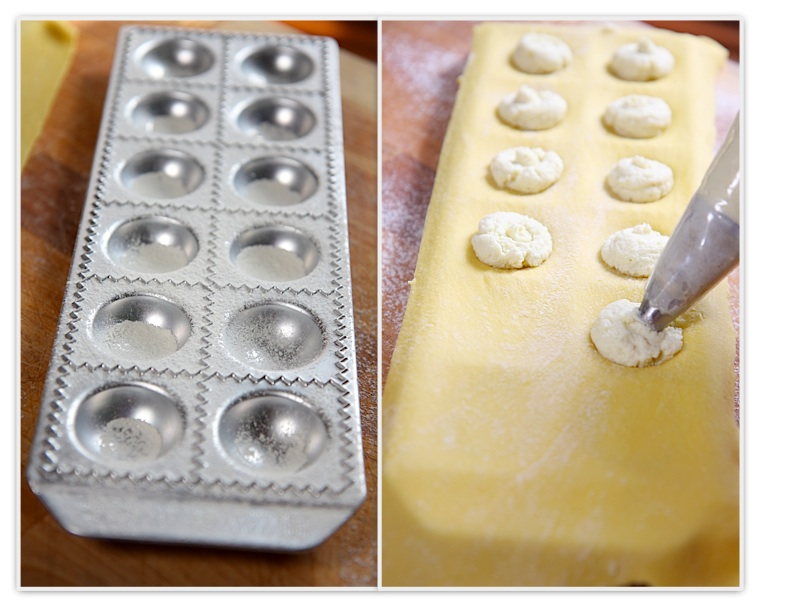
\includegraphics[scale=0.5]{images/raviolimoldwithfilling.jpg}
			\caption{Ravioliplatta för manuell fyllning av Ravioli}
			\label{ravioliplatta}	
		\end{center}
	\end{figure}
En annan typ av maskin som illustreras på figur~\ref{pastamaskin}, är väldigt stor och priset är högt som medför att de inte kan användas av hushåll.

Idén bakom detta projekt baseras på behovet av en Raviolimaskin hemma. Tanken är att utveckla en liten och relativ billig Raviolimaskin som kan vara användbar hemma.
 		\begin{figure}[h]
 			\begin{center}
 				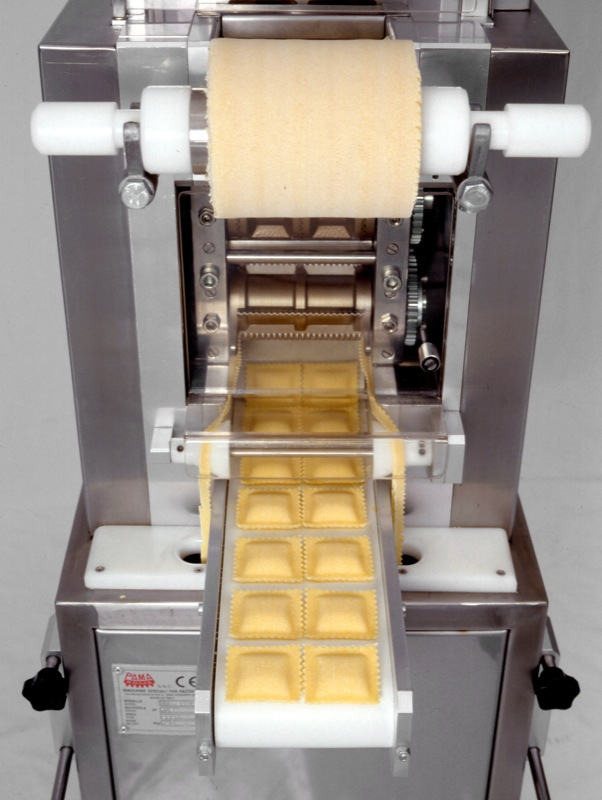
\includegraphics[scale=3]{images/pastamachine.jpg}
 				\caption{Industriell Pasta-/Raviolimaskin}
 				\label{pastamaskin}	
 			\end{center}
 		\end{figure} 

\subsection{Projektmodell} % Project model
Projektet kommer att följa den modell som presenteras i kap. 3, 

\subsection{Utvecklad produkt} % Developed product
Detta projekt är ämnat till att skapa och utveckla mjukvaran till ett cykelgarage. Den slutliga produkten ska
 tillgodose behovet av välorganiserade cykelgarage med minimala stöldrisker.

Hela systemet kommer att bestå av en operatör, där systemdatorn med programvaran och 
en streckkodutskrivare finns, som är ansluten till själva garaget. Med hjälp av operatören 
skall kunder kunna registreras/avregistrera. Varje cykel ska kunna identifieras med en 
streckkod tillhandahållen av skrivaren. Garaget ska ha en ingång med streckkodläsare, panel för 
PIN-kod och datorstyrt lås samt en utgång med streckkodläsare. Registrerade ägare ska kunna ha
 ett begränsat antal cyklar i garaget.

Ett normalt användningsscenario kan se ut enligt följande:

\begin{enumerate}
\item En cykelägare med cykel kommer till ingången.
\item Ägaren låser upp dörren genom att läsa av streckkoden på cykeln.
\item Ägaren ställer cykeln i garaget, låser den och går sen ut genom utgången.
\end{enumerate}

Samt:

\begin{enumerate}
\item En cykelägare utan cykel kommer till ingången.
\item Ägaren låser upp dörren genom att slå in sin PIN-kod.
\item Ägaren hämtar sin cykel.
\item Ägaren läser av streckkoden på cykeln vid utgången och går.
\end{enumerate}


\subsection{Syfte och Mål} % Goals
(Här beskriver du vad som är syftet med ditt projekt. Vad skall du göra? Det skall vara kortfattat (detaljer kommer i senare avsnitt).)
\\*

Detta projekts syfte är att utveckala en Ravioli maskin som (gör det mesta som en industeriell maskin gör men det ska vara)är rätt anpassad till hushåll i storleken, priset och användbarheten. Det är tänkt att användaren kan använda olika typer av ifyllnings material på maskinen.\\*

Maskinen är tänkt att göra det mesta av processen själv, genom att fylla Ravioli degar med ifyllnings material och stänger dem i slutet.



\subsubsection{Företagsmål}
För att uppmuntra användandet av cyklar som transportmedel vill företaget underlätta cykelanvändningen
 genom att erbjuda säkra, organiserade cykelgarage som inte blir överfulla. Målet är att cyklister hellre
 ska välja företagets organiserade garage framför öppna, publika cykelställen med större trängsel och
 ökad risk för stöld och vandalism.

\subsubsection{Produktmål}
Målet med produkten är att tillhandahålla säkra, organiserade cykelgarage där kunden inte behöver oroa 
sig över att cykeln står på öppen eller allmän plats. Garaget ska kräva minimal övervakning och underhåll men 
kunna identifiera de människor som kommer och går vilka cyklar de har med sig. Systemet ska även ha mycket 
hög driftssäkerhet för att undvika att kunder inte kommer åt sina cyklar.

\subsubsection{Projektmål}
Målet med detta projekt är att utveckla en effektiv och  lätt Ravioli maskin . 
Det skall vara mycket  billigare jämfört med priserna på marknaden. 

\subsection{Begränsningar} % Constraints
Eftersom existerande verktyg används är den enda stora begränsningen den tid det tar att genomföra 
projektet. Tiden är låst till en deadline som inte kan flyttas, och personalresurser är begränsade. 
Följaktligen är kvaliteten den enda variabel som kan ändras om projektet löper risk att inte bli klar 
på utsatt tid.


\section{Metod}
%Beskrivning av kunskapsläget 
%Hur uppgiften specificeras
%Metodbeskrivning
%Hur du analyserar resultatet efteråt
%Vad du skall visa på UtExpo
\section{Kunskapsläge}
\input{chapters/kunskapsläge}
\section{Projektorganisation} % Project organisation
\subsection{Utvecklingsorganisation} % Development organisation
Projektmedlemmarna är följande:

\begin{itemize}
\item Reshad Ahmadi (ansvarig för elktro samt mek delen)
\item Maryam Bayat (ansvarig för data delen)

\end{itemize}


\subsection{Intressenter} % Stakeholders
Det finns ett antal intressenter i projektet. Kursledningen agerar som den tänkta kunden som är en tågstation i södra Sverige, kap. 3 i \cite{engproc}.

\begin{itemize}
\item Kursledningen i kursen ETSA01 på LTH -- tillhandahåller simulator av hårdvaran (kursansvarig Martin Höst)
\item Projekthandledare -- mottagare av leverabler såsom dokument (Björn Regnell)
\end{itemize}

Lärarna utför acceptansprovning på den levererade produkten, för att se till att produkten uppfyller:

\begin{itemize}
\item kraven i kravspecifikationen,
\item kvaliteten på kravspecifikationen är tillräckligt bra,
\item kvaliteten på testplanen är tillräckligt bra
\item samt projektmodellen har följts.
\end{itemize}

\section{Krav på hårdvara och programvara} % Hardware and software resource requirements
Existerande verktyg och programvara kommer att användas. Öppna format och fri programvara ska användas i största möjliga mån före stängda och kommersiella system på grund av portabilitet och projektets låga budget.

\ \\

\begin{tabular}{l|l|p{3.5cm}}
\textbf{Verktyg}		&	\textbf{Syfte}	&	\textbf{Anmärkning} \\
\hline
Subversion (SVN)		 &	 Versionshantering 	&	 - \\
Eclipse		 &	 Utvecklingsmiljö för Java	 &	 SVN-plugin finns. \\
Latex 	&	 Dokumenthantering	 &	 God tillgänglighet på program. \\
Java		 &	 Kompilator och VM 	&	 - \\
Assembla		 &	 Projektverktyg online	 & 		Hosting för versionshantering. Använder delvis fri mjukvara. \url{www.assembla.com}. \\
\end{tabular}

\ \\

För testning finns simulator för hårdvara implementerad i Java.

\section{Nedbrytning av arbete} % Work breakdown
\subsection{Aktiviteter} % Activities

\begin{description}
 \item[Projektplanering] En planering utav arbetet som skall definiera uppgifter samt milstolpar i projektet.
 
 \item[Kravspecificering] Krav diskuteras, eliciteras och omformuleras.

 \item[Högnivå-design] Design av systemet för en översiktlig struktur, som resulterar i lågnivå-design senare.

 \item[Testplanering] En testplan beskriver hur programmet kommer fungera i olika testscenarion samt förhållanden.
 
 \item[Implementering] Utgående från designen sker implementeringen i programkod. Olika delar av systemet implementeras parallellt.

 \item[Kvalitetsförsäkring] När programmet är färdigskrivet måste programmet testas för att försäkra kunden att programmet uppfyller kraven ställda på kravspecifikationen.
 
 \item[Rapportering] Rapporteringen sker internt inom gruppen fär att färsäkra gruppmedlemmarna om respektive person är färdiga med sina uppgifter eller ej.
\end{description}

\subsection{Leverabler} % Deliverables

\begin{description}
 \item[Projektplan] Övergripande planen för hur projektet ska genomföras. Detta dokument. Dokumentansvarig: Johan Lundström.

 \item[Kravspecifikation] Kundens lista på specifika krav, vilket produkten begärs kunna lösa. Dokumentansvarig: Mazdak Farzone.

 \item[Design] Programdesign utifrån kravspecifikationen.
 
 \item[Programkod] Systemimplementation i Java som formar mjukvaran.

 \item[Testplan] Dokumentet som beskriver interna samt extarna tester som utförs på programmet. Dokumentansvarig: Björn Lennernäs.

 \item[Testprotokoll] Ifyllda protokoll över de tester man utfört på programvaran.
\end{description}

\section{Uppgifter}

\begin{tabular}{l|l|l|l}
\textbf{Deluppgift}		&	\textbf{Beskrivning}		&   \textbf{Tid}		&	\textbf{Krav} \\
\hline
T1 		&	Projektplan		&	8 dagar , 31/3-7/4		&	\\	
T2 		&	Kravspecifikationen		&	14 dagar , 7/4-21/4  	&	T1 \\
T3 		&	Design		&	7 dagar, 21/4-28/4		&	 T1 \\	
T4 		&	Testplan		&	7 dagar, 21/4-28/4		& 	T2 \\	
T5 		&	Kodning	  	&	14 dagar, 28/4-12/5	&	 T2 \\	
T6 		&	Testning		&	14 dagar, 4/5-18/5 	&	 T1, T5 \\	
\end{tabular}

\subsection{Milstolpar} % Milestones

\begin{itemize}
  \item Specifikationer (\emph{M1})
  \item Design (\emph{M2})
  \item Kodning (\emph{M3})
  \item Testning (\emph{M4})
\end{itemize}



\subsection{Tidplanering} % Scheduled and estimated effort

\section{Uppföljning, rapportering och kvalitetssäkring} % Monitoring, reporting and quality assurance
Gruppen ser till att mötas regelbundet. På mötena granskas arbete utfört av gruppmedlemmar, speciellt inför
varje extern granskning av gruppens handledare så granskar gruppen de dokument eller program som 
skall lämnas in till handledaren och avgör om de behöver kompletteras eller ej. Handledaren godkänner kvaliten på
arbetet eller ber om komplettering. På mötena utses även ansvariga för olika delar av projektet, samt vilka som skall 
arbeta på vilket dokument eller program. Ansvaret ligger sedan hos den ansvariga för dokumentet/programmet att se till
att de arbetare personen har tillgång till utför ett effektivt arbete, och att arbetet är slutfört inför nästa deadline.

Gruppen använder sig av projektverktyget Assembla som är speciellt utvecklat för programvaruutveckling. 
Webbsidan ger bland annat tillgång  till ett antal viktiga verktyg för konfigurationshantering och intern rapportering.
Gruppens dokument och program är kan laddas upp på sidan, där samtliga medlemmar i gruppens tillåts ändra dokumenten
och programmen. Ändringarna kommenteras av den som utfört ändringen och både det som ändrats på och den nya 
versionen av dokument eller programmet sparas. På så sätt  upprätthålls en meningsfull dialog för ändringar i dokumenten/programmen
samt att alla versioner av dokumentet kan återskapas. 

På webbsidan upprätthåller gruppen även uppgifter om vem som skall göra vad och när det skall vara klart, samt andra viktiga 
tidpunkter och uppgifter som var och när nästa möte skall hållas och hur medlemmarna skall förbereda sig inför detta möte. Webbsidan möjliggör även en
kommunikation mellan olika medlemmar i gruppen, där de olika medlemmarna kan rapportera till exempelvis en ansvarig för ett visst
dokument/program vad som gjorts, av vem och vad som återstår att göra.


\section{Riskanalys}

\begin{description}
\item[Projektdeltagare tillgänglighet:]
En eller flera nyckelpersoner i gruppen blir sjuka eller har hög frånvaro. \\
\emph{Sannolikhet:}
Medel \\
\emph{Effekt:}
Hög \\
\emph{Strategi:}
Genom kontinuerlig kommunikation och kunskapsspridning inom gruppen kan detta
undvikas. \\
\emph{Riskindikator:}
Risken kan upptäckas vid bortfall av gruppmedlemmar på möten och att 
deluppgifter inom projektet inte blir genomförda i tid.

\item[Kravförändringar:]
Förändring eller missförstånd av krav i kravspecifikationen för projektet kan
 innebära problem längre fram vid tester av mjukvaran. \\
\emph{Sannolikhet:}
Låg \\
\emph{Effekt:}
Hög \\
\emph{Strategi:}
Kravspecifikationen bör utarbetas grundligt för att minimera att risken skall
 ske. \\
\emph{Riskindikator:}
Vid systemtest och övriga tester kan risken upptäckas.

\item[Organisation:]
Beslutsfattandet från projektledarens sida är bristfällig, vilket kan medföra
 osäkerhet i arbetet för alla projektdeltagare. \\
\emph{Sannolikhet:}
Låg \\
\emph{Effekt:}
Medel \\
\emph{Strategi:}
Genom kontinuerlig kommunikation inom gruppen och rapportering till
 projektledaren kan effekterna minimeras. \\
\emph{Riskindikator:}
Risken kan upptäckas vid dålig organisation av möten och om deluppgifter inom
 projektet börjar bli osammanhängande på grund av bristande kommunikation
 mellan projektdeltagare.

\item[Tidsuppskattning:]
Dålig uppskattning av tidsupptagandet för delmoment inom projektet kan försena
 hela projektet. \\
\emph{Sannolikhet:}
Medel \\
\emph{Effekt:}
Hög \\
\emph{Strategi:}
Fortlöpande kommunikation och rapportering av delmoment inom projektet mellan
 projektledaren och projektdeltagare skall minimera eventuella
 tidsförseningar. \\
\emph{Riskindikator:}
Risken kan upptäckas vid försening av deluppgifter.

\item[Problem med mjukvara:]
Vid tester av mjukvara kan rapportering av problem uppkomma. \\
\emph{Sannolikhet:}
Medel \\
\emph{Effekt:}
Medel \\
\emph{Strategi:}
Ständiga tester av mjukvara skall genomföras för problemfri försäkran. \\
\emph{Riskindikator:}
Vid diverse tester av mjukvara kan risken påträffas.

\item[Tekniska kommunikationsproblem:]
Att vår kommunikationscentral över internet kraschar. \\
\emph{Sannolikhet:}
Låg \\
\emph{Effekt:}
Hög \\
\emph{Strategi:}
Om detta händer så kommer kommunikationen ändå fortsätta över internet fast
 utanför vår kommunikationscentral. \\
\emph{Riskindikator:}
Risken kan upptäckas vid störningar med kommunikationscentralen, att hemsidan
 inte fungerar helt korrekt.
 
 \item[Problem med mjukvara:]
Medlemmar saknar eller får problem med mjukvaran/projektverktyget. \\
\emph{Sannolikhet:}
Medel \\
\emph{Effekt:}
Låg \\
\emph{Strategi:}
En övergripande utbildning av gruppmedlemmar minskar sannolikheten att missförstånd och förseningar uppstår. \\
\emph{Riskindikator:}
Risken upptäcks exempelvis när medlemmarna engagerar sig för lite eller när en ny version av en mjukvara släpps.
\end{description}
\section{Referenser}
\section{Referenser}
\renewcommand*{\refname}{}
\vspace{-1cm} % Återställ utrymme

\begin{thebibliography}{99}
\bibitem{engproc} \emph{http://www.wisegeek.com/what-is-ravioli.htm}
\end{thebibliography}


\end{document}                 % The input file ends with this command.